% !Mode:: "TeX:UTF-8"
% !TEX program  = xelatex
\documentclass[a4paper]{article}
\usepackage{amsmath}
\usepackage{amssymb}
\usepackage{ctex}
%\usepackage{braket}
%\usepackage[european]{circuitikz}
\usepackage{multirow}
\usepackage{float}
\usepackage{graphicx}
\usepackage{geometry}
\geometry{left=2.5cm,right=2.5cm,bottom=2.5cm,top=2.5cm}
\title{近代物理实验报告3.4:单光子计数}
\author{xy
\quad 学号\quad 匡亚明学院}
\date{2019年2月29日}
\begin{document}
\maketitle
\bibliographystyle{unsrt}
%--------main-body------------

\section{引言}
通常在一些基本的科研领域,特别是某些前沿学科,诸如高分辨光谱学、非线性光学、拉曼光谱学、表面物理学的研究方面,都会遇到极微弱的光信息(简称弱光)检测问题。所谓弱光是指光流强度比光电倍增管本身的热噪声(10$^{-14}$W)还要低,以致用一般的直流检测方法已经很难从这种噪声中检测出信号。

单光子计数是目前测量弱光信号最灵敏和有效的实验手段,这种技术中,一般都采用光电倍增管作为光子到电子的变换器(近年来,也有用微通道板和雪崩光电二极管的),通过分辨单个光子在光电倍增管激发出来的光电子脉冲,利用脉冲高度甄别技术和数字计数技术,把光信号从热噪声中医数字化的方式提取出来。与模拟检测技术相比,单光子计数技术有如下的有点:
\begin{enumerate}
\item 消除了光电倍增管高压直流漏电流和各倍增极的热发射噪声的影响,提高了测量的信噪比。
\item 时间稳定性好。在单光子计数系统中,光电倍增管漂移、系统增益的变化,零点漂移和其它不稳定因素对计数影响不大。
\item 可输出数字信号,能够直接输出给计算机进行处理。
\item 有比较宽的线性动态范围,最大计数率可达10$^6s^{-1}$。
\item 有很高的探测灵敏度,目前一般的光子计数器探测灵敏度优于10$^{-17}$W,这是其它探测方法达不到的。
\end{enumerate}

\section{实验目的}
\begin{enumerate}
\item 了解单光子计数工作原理。
\item 了解单光子计数器的主要性能,掌握其基本操作方法。
\item 了解用单光计数器系统结检测微弱光信号的方法。
\end{enumerate}

\section{实验仪器}
单光子计数实验系统由单光子计数器、外光路、制冷系统和电脑控制软件等组成。

\section{实验原理}
\subsection{光子流量和光流强度}
光是由光子组成的光子流,单个光子的能量$\epsilon$与光波频率$\nu$的关系是
\begin{equation}
\epsilon = h\nu = \frac{hc}{\lambda}\label{eq1}
\end{equation}
光子流量可用单位时间通过的光子数R表示,光流强度是单位时间内通过的光能量,常用光功率P表示。单色光的光功率P与光子流量R的关系是
\begin{equation}
P = R\epsilon\label{eq2}
\end{equation}
当光流强度小于10$^{-16}$W时通常称为弱光,此时可见光的光子流量可降到1ms内不到1个光子,因此实验中要完成的将是对单个光子进行检测,进而得出弱光的光流强度,这就是单光子计数。

将单位时间内通过某一截面的光子数 称为光子流量。并进一步将单位时间内通过该截面的光能量定义为光流强度,用光功率 表示。当光流强度小于 时,该束光被称为弱光。此时,可见光的光子流量可降到一毫秒不到一个光子。因此本实验中将要完成的是对单个光子进行检测,进而得出弱光的光流强度,这就是单光子计数。

\subsection{测量弱光时光电倍增管的输出特性}
光电倍增管在实验1.2中已经介绍,其结构原理如图(\ref{fig1})所示。
\begin{figure}[!h]
\centering
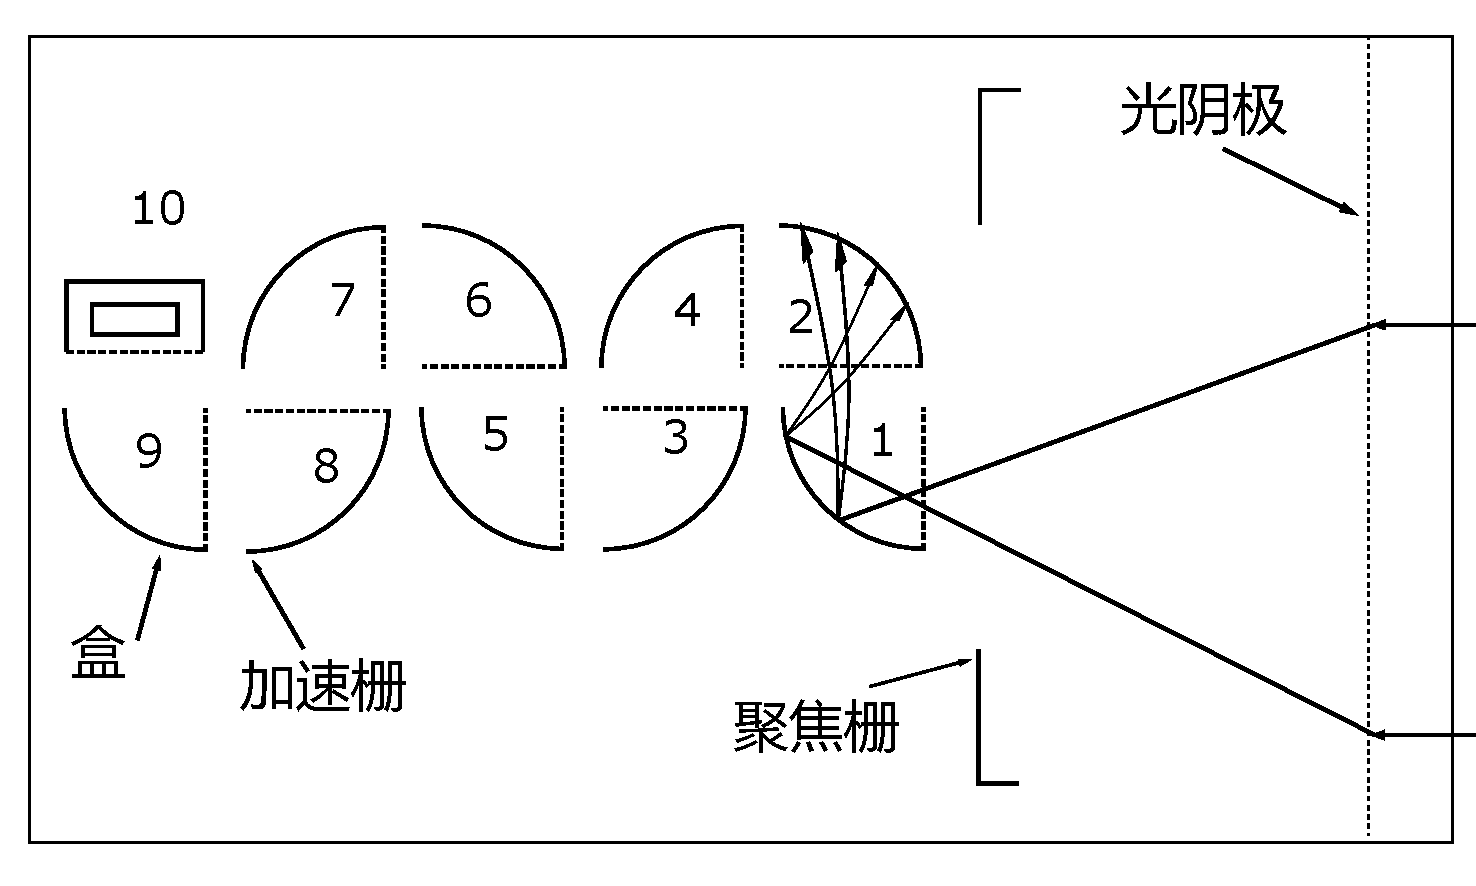
\includegraphics[width=0.9\textwidth]{fig/fig1.pdf}\\
\caption{盒栅式光电倍增管}\label{fig1}
\end{figure}

当光子入射到光电倍增管的光阴极上时,光阴极吸收光子后将发射出一些光电子,光阴极产生的光电子数与入射到光阴极上的光子数之比称为量子效率。大多数材料的量子效率都在30\%以下。咋弱光下光电倍增管输出的光电子脉冲基本上不重叠,所以光子计数实际上是将光电子产生的脉冲逐个记录下来的一种探测技术。当然,从统计意义上说也是单光子的计数。

如图(\ref{fig1})所示,光阴极上发射的光电子,经聚焦合和加速打到第一倍增极上,将在第一倍增极上打出几倍于入射电子数目的二次电子。这些二次电子被加速后打到第二倍增极上,……接连经经过十个倍增极的增殖作用后,电子数目最高可达10$^8$。最后由阳极收集所有的电子,在阳极回路中形成一个电脉冲信号,如图(\ref{fig2})所示,
\begin{figure}[!h]
\centering
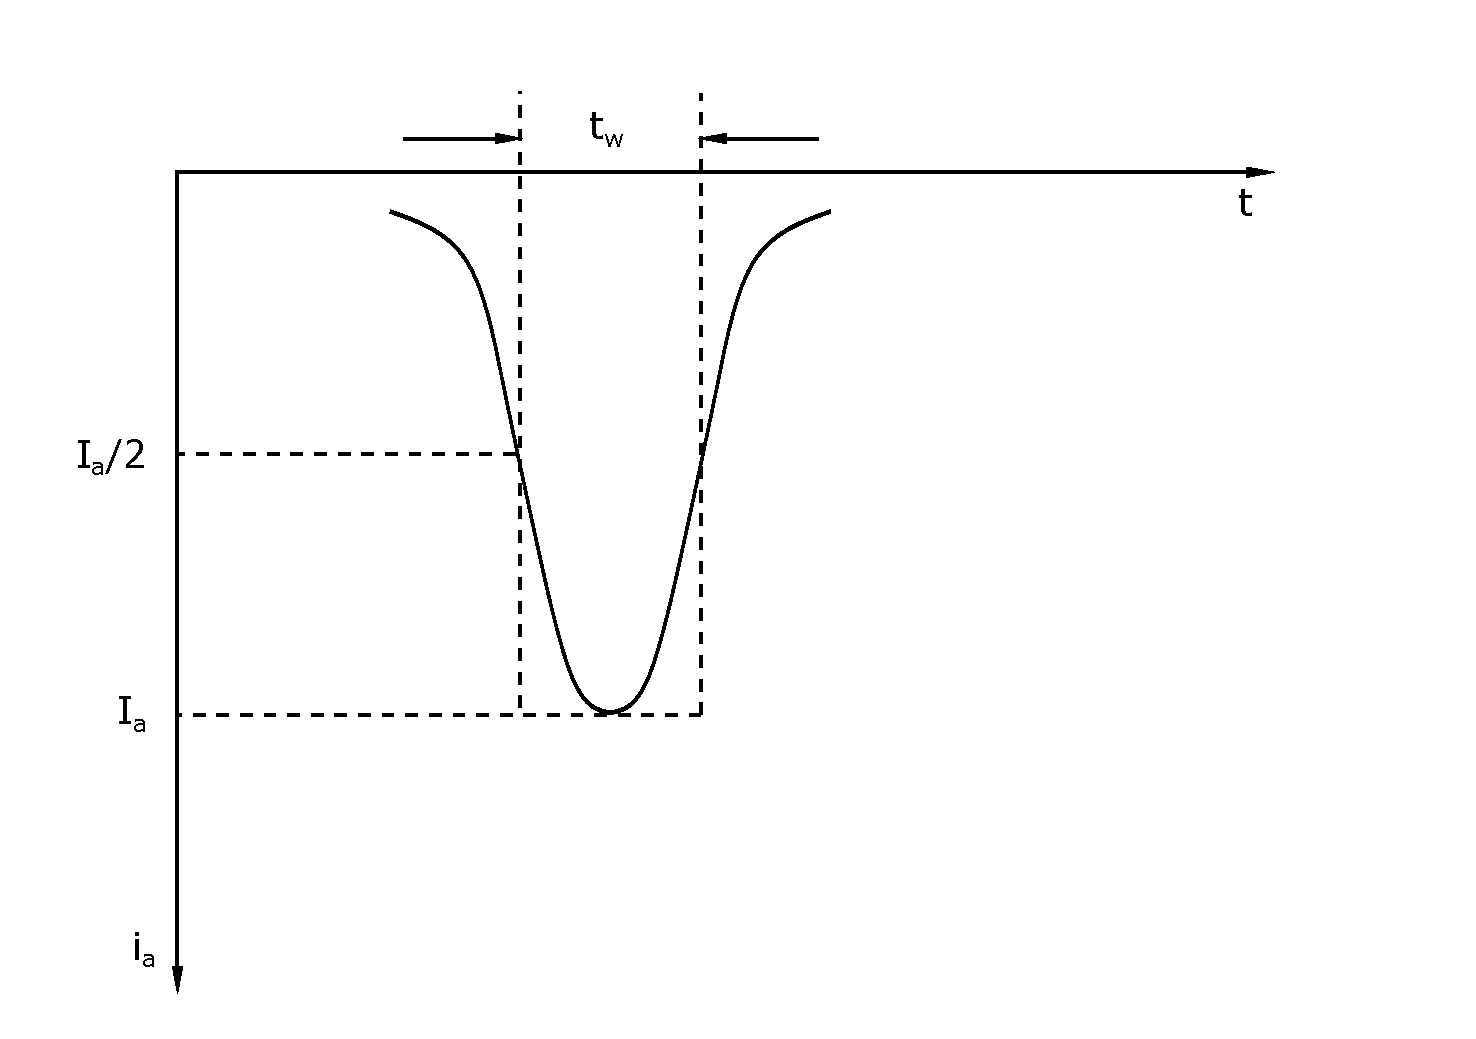
\includegraphics[width=0.8\textwidth]{fig/fig2.pdf}\\
\caption{光电倍增管阳极波形}\label{fig2}
\end{figure}
脉冲宽度$t_w$与光电倍增管的时间特性以及阳极回路的时间常数$R_LC$有关(C为阳极回路的分布电容与放大器的输入电容之和)。性能良好的光电倍增管配合以尽可能小的$R_LC$,可使脉冲宽度只有10$\sim$30ns。

当光流强度约10$^{-13}$W时,光电子信号是在直流电平上叠加闪烁噪声;当光流强度约10$^{-14}$W时,直流电平开始减小,脉冲重叠减少,但仍存在基线起伏;当光流强度约10$^{-15}$W时,基线开始稳定,重叠脉冲极少;当光流强度约10$^{-16}$W时,脉冲无重叠,基线趋于平直(如图。可见当光强降到10$^{-16}$W时,尽管光信号是由一连续发光的光源发出的,而光电倍增管输出的电信号却是一个一个分离的尖脉冲,光子流量与这些脉冲的平均计数率成正比。只要用计数的方法测出单位时间按内的光电子脉冲数,就相当于检测了光的强度。

\subsection{单光电子峰}
将光电倍增管的阳极输出脉冲接到脉冲高度记录仪器(例如多道分析器)作脉冲高度分布分析(PHA),可以得到如图(\ref{fig4})所示的分布。
\begin{figure}[!h]
\centering
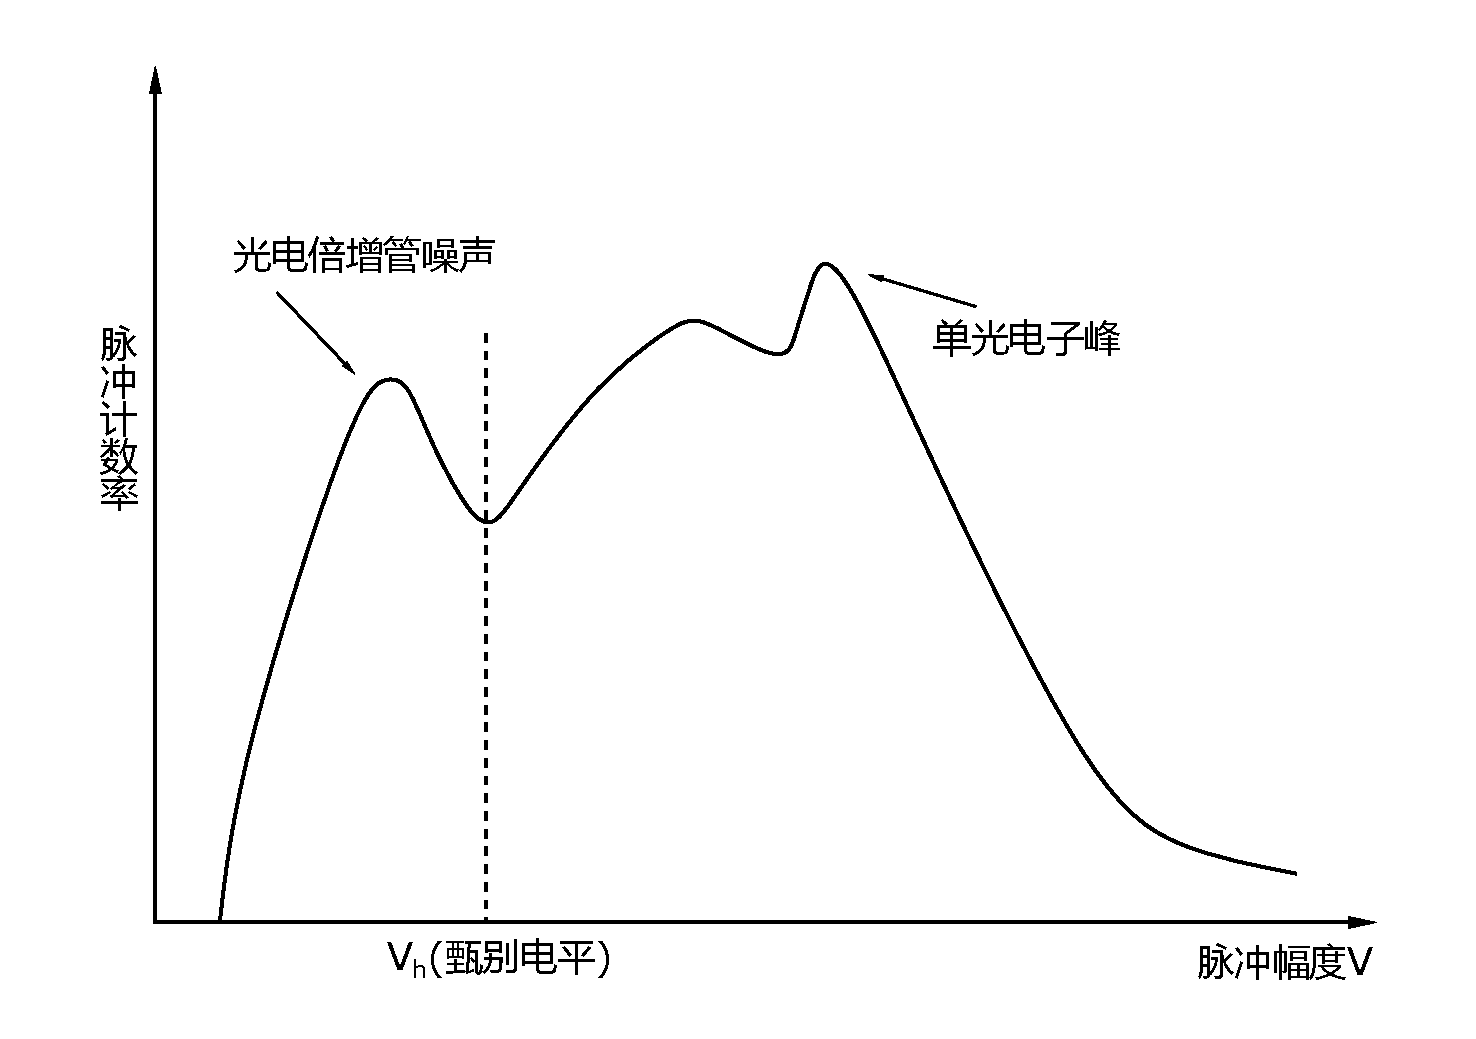
\includegraphics[width=0.9\textwidth]{fig/fig4.pdf}\\
\caption{光电倍增管输出脉冲幅度分布(微分)曲线}\label{fig4}
\end{figure}

图中曲线表明:脉冲幅度大小在V到(V+$\Delta$V)之间的脉冲计数率R与脉冲幅度大小V之间的关系。它与($\frac{\Delta R}{\Delta V}$)-V曲线由相同的形式,因此当$\Delta$V取值很小时这种幅度分布曲线称为脉冲幅度分布的微分曲线。由图中可以看出,脉冲幅度较小的主要是热发射噪声信号,而光阴极发射的电子形成的脉冲,其幅度集中在横坐标的中部,形成所谓的“单光电子峰”。
形成这种分布的主要原因是:
\begin{enumerate}
\item 光阴极发射的电子,包括光电子和热发射电子,都受到了所有倍增极的增殖。因此它们的幅度大致接近。
\item 各倍增极的热发射电子经受倍增的次数要比光阴极发射的电子经受的少,因此前者在阳极上形成的脉冲幅度要比后者低。所以,图(\ref{fig4})中脉冲幅度较小的部分主要是热噪声脉冲。
\item 各倍增极的倍增系数不是一定值,有一统计分布,大体上遵守Poisson分布。
\end{enumerate}
所以,如果用脉冲高度甄别器将幅度高于图(\ref{fig4})中谷点的脉冲加以甄别、输出并计数显示,就可实现高信噪比的单光子计数,大大提高检测灵敏度。

\subsection{光子计数器的组成}
光子计数器的原理方框图如图(\ref{fig5})所示,各部分功能和主要要求如下:
\begin{figure}[!h]
\centering
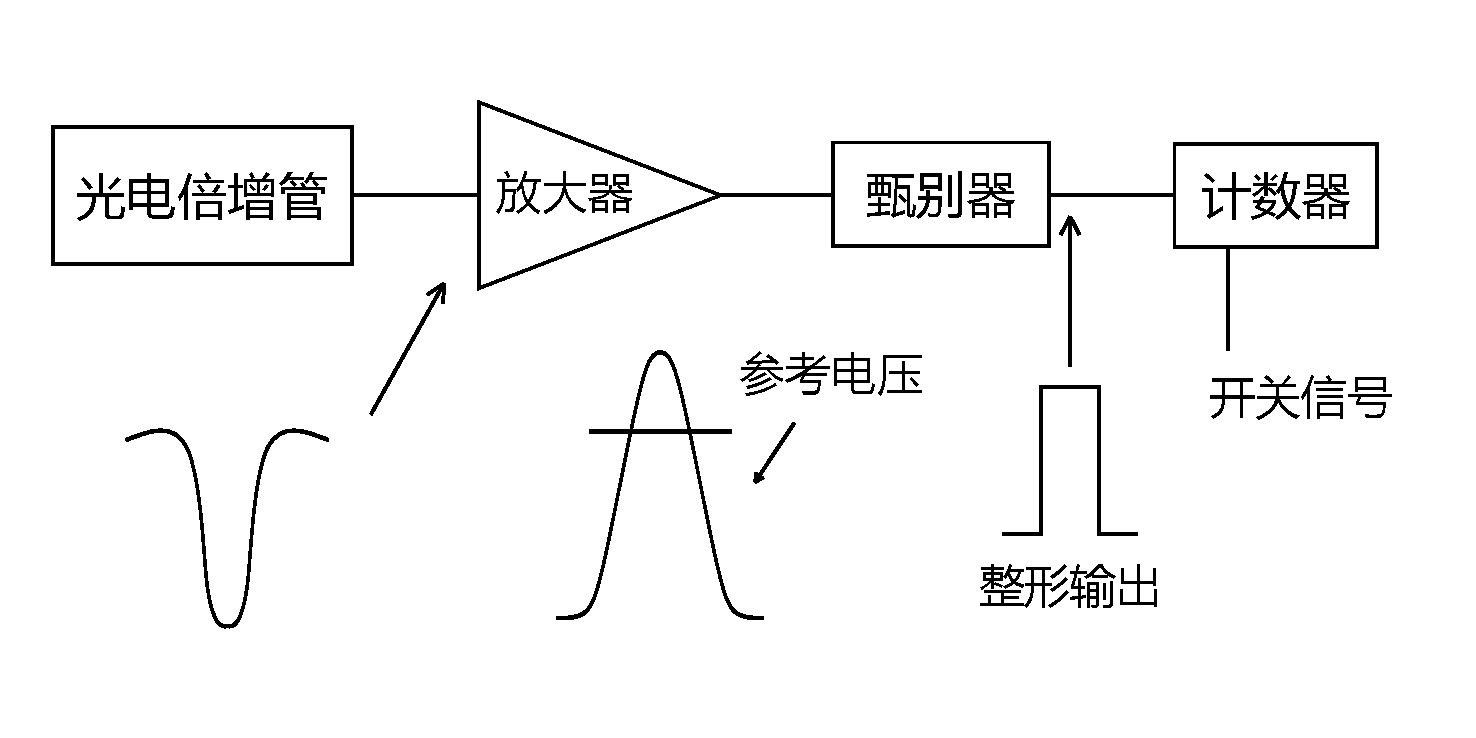
\includegraphics[width=0.9\textwidth]{fig/fig5.pdf}\\
\caption{光子计数器方框图}\label{fig5}
\end{figure}

\subsubsection{光电倍增管}
由以上分析可知,能够进行光子计数的一个重要条件是要有性能良好的光电倍增管。更具体地说,用于光子计数的光电倍增管必须具有适合于实验中工作波段的光谱响应,要有适当的阴极面积,量子效率高,暗计数率低,时间响应快,并且光阴极稳定性高。为了获得较高的稳定性,除尽量采用光阴极面积小的管子外,还采用致冷技术来降低管子的环境温度,以减少各倍增极的热电子发射。
\subsubsection{放大器}
放大器的作用是将光电倍增管阳极回路输出的光电子脉冲(连同其他噪声脉冲)线性地放大。放大器的增益可根据单光电子脉冲的高度和甄别器甄别电平的范围来选定。另外还要求放大器具有较宽的线性动态范围,上升时间$\leq$3ns(即通频带宽超过100MHz),噪声系数小等。光电倍增管与放大器的连线应尽量短以减少分布电容,有利于光电脉冲的形成与传播。
\subsubsection{脉冲高度甄别器}
脉冲高度甄别器的作用是鉴别输出光电子脉冲,弃除热发射噪声脉冲。它有连续可调的阈电平,称甄别电平。只有当输入脉冲的幅度大于甄别电平时,甄别器才输出一个有一定幅度和形状的标准脉冲(如图(\ref{fig6}))。
\begin{figure}[!h]
\centering
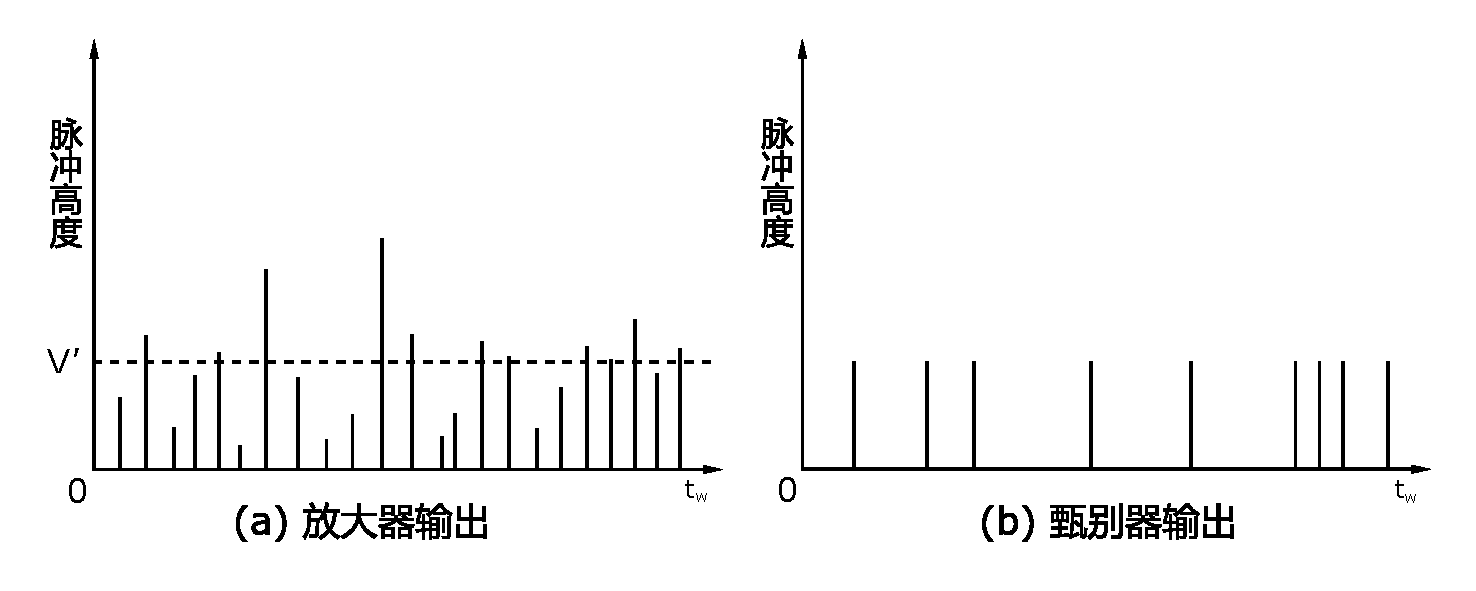
\includegraphics[width=0.9\textwidth]{fig/fig6.pdf}\\
\caption{甄别器工作示意}\label{fig6}
\end{figure}
在用于光子计数时,可以将甄别电平调节到图(\ref{fig6})中单光电子峰的下限处。这时各倍增极所引起的热噪声脉冲因小于甄别电平而不能通过。经甄别器后只有光阴极产生的光电子脉冲和热电子脉冲的输出。

对甄别器的要求是甄别电平稳定,灵敏度高,死时间小。当有一脉冲触发了甄别器中的线路后,在它恢复原状以前甄别器不能接受后续脉冲,这段时间按称为死时间,用于光子计数的甄别器的死时间要求小于10ns。
\subsubsection{计数器}
计数器(或称定标器)的作用是将甄别器的输出的脉冲累积起来并予以显示。用于光子计数的计数器要满足高技术率的要求,即要能够分辨时间间隔为10ns的二脉冲,相应的计数率为100MHz。不过当光子计数器用于微弱光的测量时,它的计数率一般很低。因此采用计数率低于10MHz的计数器亦可。这部分还必须有控制计数时间的功能。
\subsection{光子计数器的噪声和信噪比}
光子计数器的噪声来源主要为光子发射的统计涨落、光阴极和倍增极的热电子发射和脉冲堆积效应等。
\subsubsection{统计涨落噪声}
就热光源来说,在发光时各原子是相互独立的,相继的两个光子打到光阴极上的时间间隔是随机的。按照统计规律在一定的时间间隔t内发出的光子数服从Poisson分布。
\subsubsection{暗计数噪声}
由于光电倍增管的光阴极和各倍增极有热电子发射,即使入射光强为0时,还有暗计数,也称本底计数。通常采用降低管子的工作温度,选用小面积光阴极和选择合适的甄别电平等措施,力图使暗计数率$R_d$降到最小。但对于极微弱的光信号,暗计数仍是一个不可忽略的噪声来源。
\subsubsection{脉冲堆积效应噪声}
分析光子计数器的噪声和计数误差时,除上述几个重要因素外,还应考虑脉冲堆积效应。这是计数率较高时的主要误差来源。

光电倍增管输出的脉冲有一定的宽度$t_w$,只有在从一个光电子脉冲产生时算起,经过比$t_w$更长的时间间隔后,光电倍增管阳极回路才能接着输出另一个光电子脉冲,$t_w$称为光电倍增管的分辨时间。当后续光电子脉冲与前一个脉冲的时间间隔小于$t_w$时,阳极回路只输出一个脉冲,这现象称为脉冲堆积效应。如果接连有很多脉冲来临前的时间间隔都小于$t_w$,这些脉冲都不能分辨。可见,光电倍增管也具有死时间。在这意义下光电倍增管被称为“可瘫痪”的探测器,就是说它的计数率有上限,超过此上限就出现计数率的损失。

\section{实验内容}
\subsection{观察不同入射光时放大器和甄别器输出脉冲的波形特征,并做比较}
\begin{enumerate}
\item 开启GSD-2单光子计数实验仪“电源”(位于仪器的左边),光电倍增管预热30分钟。
\item 开启“功率测量”在$\mu$W量程进行严格调零;开启“光源指示”,电流调到1mA$\sim$4mA,读出“功率测量”指示的P值。
\item 开启微机,运行“单光子计数”软件,给光电倍增管提供工作电压,探测器开始工作。
\item 开启示波器,调节“触发电平”处于最灵敏状态。分别将放大器输出信号(检测2)和甄别器输出信号(检测1)馈送至示波器的输入端,观察并记录两种信号的波形特征。
\item 由大到小的顺序依次减低供给光源的电流,观察示波器上上述两种波形的变化。图形应该是由连续谱变为离散的尖脉冲。
\end{enumerate} 
\subsection{测量光电倍增管输出脉冲幅度分布的积分和微分曲线,确定测量弱光时的最佳阈值(甄别)电平$V_h$,并记录最佳阈值}
\begin{enumerate}
\item 选择光电倍增管输出的光电信号是分立尖脉冲的条件,运行“单光子计数”软件。在模式栏选择“阈值方式”;采样参数栏中的“高压”是指光电倍增管的工作电压,1$\sim$8档分别对应620$\sim$1320V,由高到低每档10\%递减。
\item 在工具栏点击“开始”获得积分曲线。视图形的分布调整数值范围栏的“起始点”和“终止点”,“终止点”一般设在30$\sim$60档左右(10mV/档);再适当的调整光电倍增管的高压档次(6$\sim$8档范围)和微调入射光强,让积分曲线图形为最佳(如图(\ref{fig12}))。
\begin{figure}[!h]
\centering
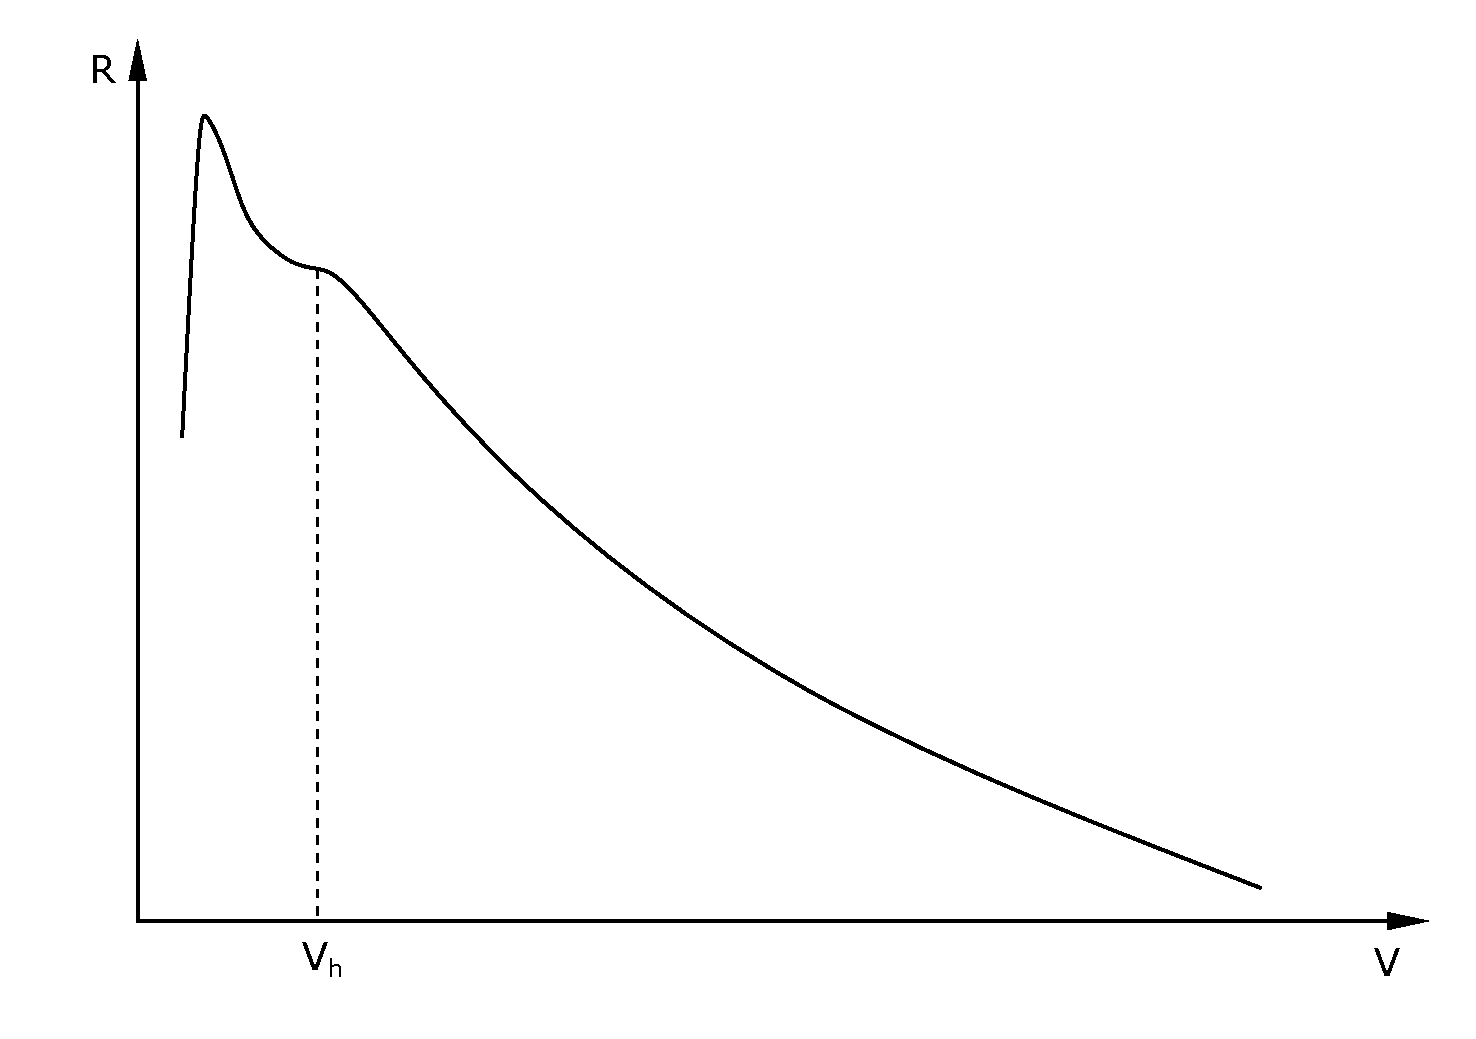
\includegraphics[width=0.6\textwidth]{fig/fig12.pdf}\\
\caption{输出脉冲分布(积分)曲线}\label{fig12}
\end{figure}

其斜率最小值处就是阈值电平$V_h$。
\item 在菜单栏点击“数据/图形处理”选择“微分”,再选择与积分曲线不同的“目的寄存器”运行,就会得到与积分曲线色彩不同微分曲线。其电平最低谷与积分曲线的最小斜率处相对应,由微分曲线更准确的读出$V_h$。
\end{enumerate}
\subsection{测量接收光功率,求信噪比}
\begin{enumerate}
\item 由模式栏选择“时间方式”,在采样参数栏的“域值”输入步骤2获取的$V_h$值,数值范围的“终止点”不用设置太大,50$\sim$100即可,在工具栏点击“开始”,单光子计数。将数值范围的“最大值”设置到单光子数率线在显示区中间为宜。 
\item 此时,如果光源强度P不变,光子计数率$R_P$基本是一直线;倘若调节光功率P的高、低,光子数率也随之高、低而变化。这说明:一旦确立阈值甄别电平、测量时间间隔相同,P与$R_P$成正比。测量三种不同光功率(在1$\mu$W以上)的光计数$N_t$和无光时的暗计数$N_d$(可从计数率曲线上取5点的数值,平均而得),计算出接收光功率$P_i$。
接收光功率$P_i$和信噪比SNR可分别按下述方法计算:
\begin{equation}
P_i = \cfrac{E_pR_p}{\eta}\label{eq4}
\end{equation}
其中$E_p$=3.96×10$^{-19}$J(500nm波段光子的能量),$R_P$为计数率,等于光计数率$N_p$除以积分时间,CR125型光电倍增管对500nm波段的量子计数效率$\eta$=15\%。
\begin{equation}
\text{SNR} = \cfrac{N_t - N_d}{\sqrt{N_t + N_d}}\label{eq5}
\end{equation}
式中,$N_t$为测量时间间隔内测得的总计数,$N_d$为测量时间间隔内测得的背景计数。光计数$N_p = N_t - N_d$。
\end{enumerate}

\section{实验数据}

\section{实验讨论与误差分析}

\section{思考题}
\subsection{为什么由持续照射的光源得到的弱光信号可以用脉冲计数的方法检测?}
答:弱光信号的光流强度小于 ,此时尽管光信号是一连续发光的光源发出的,但光电倍增管输出的电信号却是一个一个分离的尖脉冲,光子流量与这些脉冲的平均计数率成正比。所以只要用计数的方法测出单位时间的光电子脉冲数,就相当于检测了光的强度。

\subsection{测得的接收光功率 与推算的入射光功率 是否一致?若不一致,试分析其原因。}
答:不一致。而且相对误差达到或超过 。
尝试讨论原因如下:
1)	未预热,导致仪器工作状态不稳定。
2)	推算公式中的各项常数可能与真实值有较大偏差,毕竟仪器经过长时间使用,一些基本参数有所改变也是正常现象。
3)	由于脉冲堆积效应导致计数减少,进而使测得的接收功率偏小。不过如此大的误差来源于此的话,就是说未计数的光子的是已计数的光子数量的4倍到5倍。当然随着电流增大误差越来越大的现象,倒是与脉冲堆积效应导致误差可能产生的结果一致。

\nocite{jiaocai}
\bibliography{ref}
\end{document}